% !TeX root = ../thuthesis-example.tex

\chapter{Introduction}

In 1985 Kary Mullis revolutionised the nucleic acid research field with the Nobel awarded Polymerase Chain Reaction (PCR) technique \cite{saiki_enzymatic_1985}. Since that moment humankind was able to replicate \emph{in vitro} the first step of the biology central dogma, making it possible to amplify, detect and even edit DeoxyriboNucleic Acid (DNA). Later, PCR has been the precursor of a long family of nucleic acid amplification procedures that have taken one step further the capabilities of the technique.

Diagnostics and biosensing are some of the most affected fields by the PCR invention. As a Nucleic Acid Amplification Test (NAAT), and in contrast with other non-nucleic-acid based techniques, PCR has the key advantage of replicating one of the molecules present in the target, and therefore, generating a highly specific exponential signal. In the end, this allows NAATs to reach robust levels of sensibility and specificity. 

Even though PCR-based NAATs have become the gold standard in the biosensing field\cite{oliveira_isothermal_2021}, they have a main limiting factor; they require a highly expensive environment to perform accurately, including a fully equipped molecular lab and well-trained personnel. 
\linebreak
\linebreak

\begin{figure}[b]
    \centering
    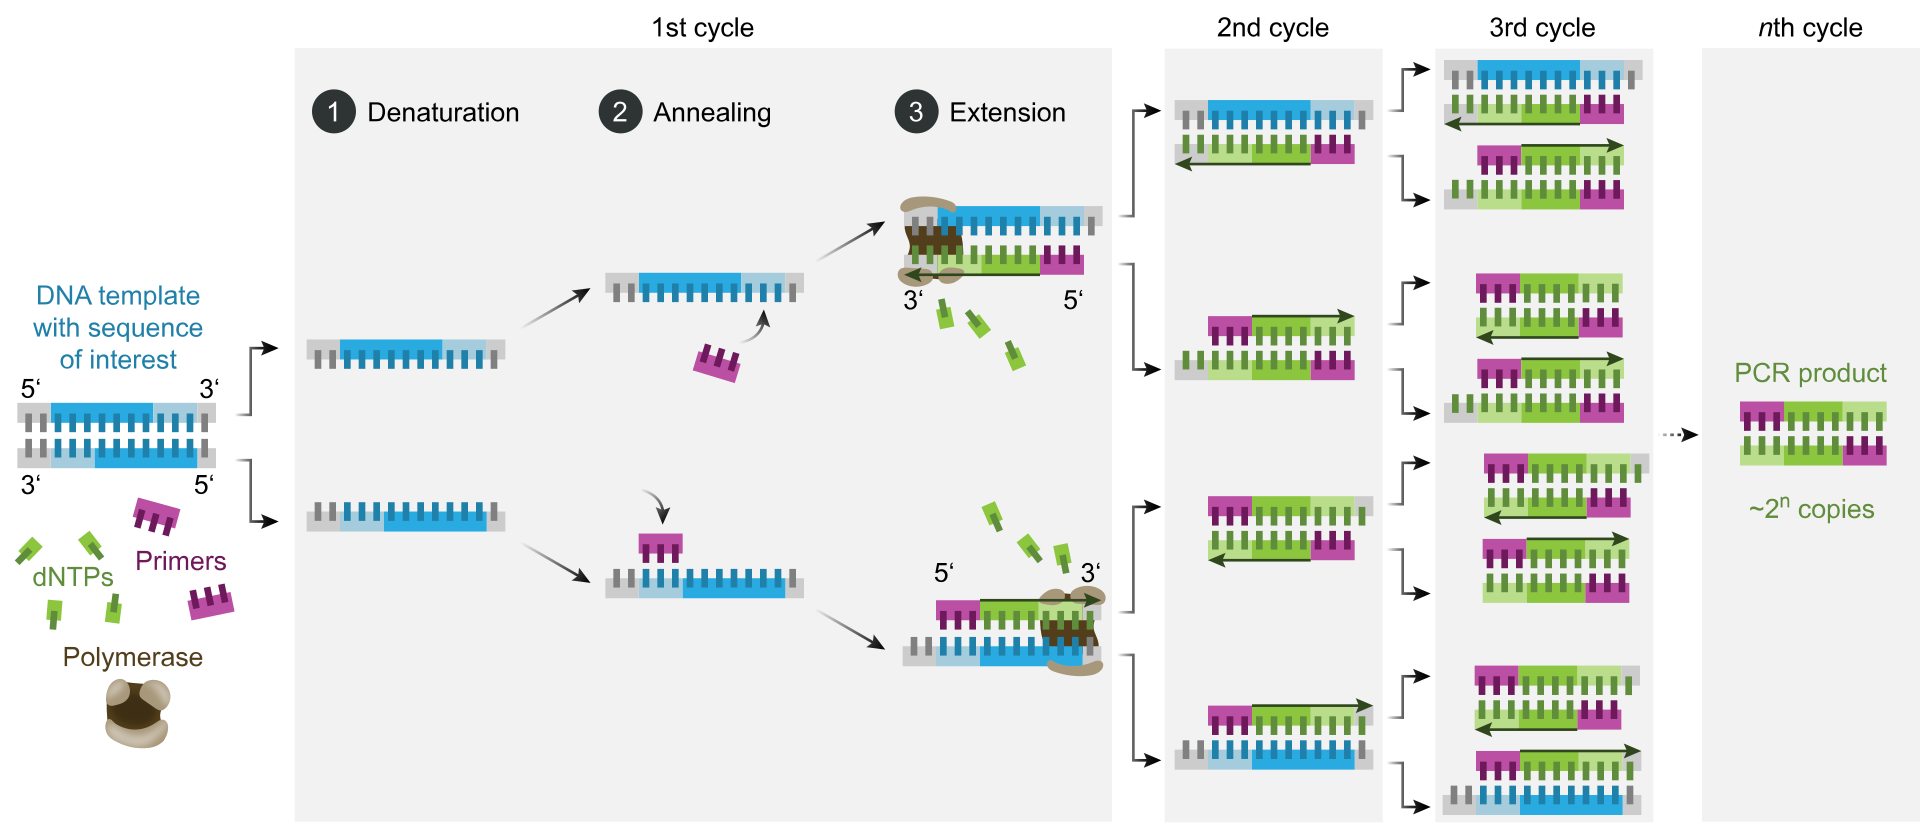
\includegraphics[width=1\textwidth]{figures/PCR.png}
    \caption[Scheme of PCR amplification working principle.] {Scheme of PCR amplification working principle. Adapted from Enzoklop, CC BY-SA 4.0 , via Wikimedia Commons.}
    \label{fig:PCR}
\end{figure}


\section{The problem of thermal cycling}

Through the PCR, the reactions are submitted to cycles of heat and cold, which helps couple and uncouple the double strand of nucleic acids and create the conditions that the reagents need to interact with the DNA. 

When it comes to diagnosis the gold standard is Real-Time PCR (RT-PCR)\cite{world_health_organization_laboratory_2016}\cite{world_health_organization_interim_2015}\cite{world_health_organization_recommendations_2021}. The RT-PCR is an evolution of PCR, where the amplification of DNA is designed to give a fluorescent signal that is measured cyclically during the reaction. The amount of signal at a certain time is proportional to the initial quantity of target in the sample, and therefore, the amount of target can be quantified by comparing the signal with the fluorescence of a control.For carrying out the amplification, a \emph{thermocycler} is required, which provide fast temperature switching making the system efficient and drastically reducing the required time. In the case of RT-PCR, the machine used is called \emph{Real-Time thermocycler}, which additionally measures the signal fluorescence cyclically. Standard Real-time thermocyclers cost around 40.000\$, are not portable and their use requires specialized molecular biology training.

All of these ends up generating so many difficulties to implement these technologies for diagnoses in Low to Middle-Income Countries (LMIC), where, paradoxically, they are more needed.

\section{The isothermal Nucleic Acid Amplification Tests}

In a nutshell, the isothermal Nucleic Acid Amplification Test (iNAAT) are  NAATs that happen at a constant temperature. This key factor generates a huge improvement in the applicability of the PCR-based NAATs because there is no longer a need for a thermocycler and the reactions can be carried out just in a simple water bath or incubator. 

Even if initially it might appear challenging, nature always works amplifying nucleic acids at a constant temperature. Indeed, this technology replicates solutions that are already present in nature to solve the strand unfolding challenge. Contrary to current thinking, the isothermal amplifications preceded the invention of PCR. In 1965 Spiegelman laboratory used purified RNA-dependent-RNA-polymerase from the bacteriophage Qbeta (Qb) to exponentially amplify the phage genome \emph{in vitro} \cite{spiegelman_synthesis_1965}. The group later discovered that this method generates the accumulation of numerous errors, which led this technique to be used as the first attempt for extracellular evolution. However, when it comes to efficient DNA amplification, the technique was later on completely eclipsed by PCR.

\begin{figure}[b]
    \centering
    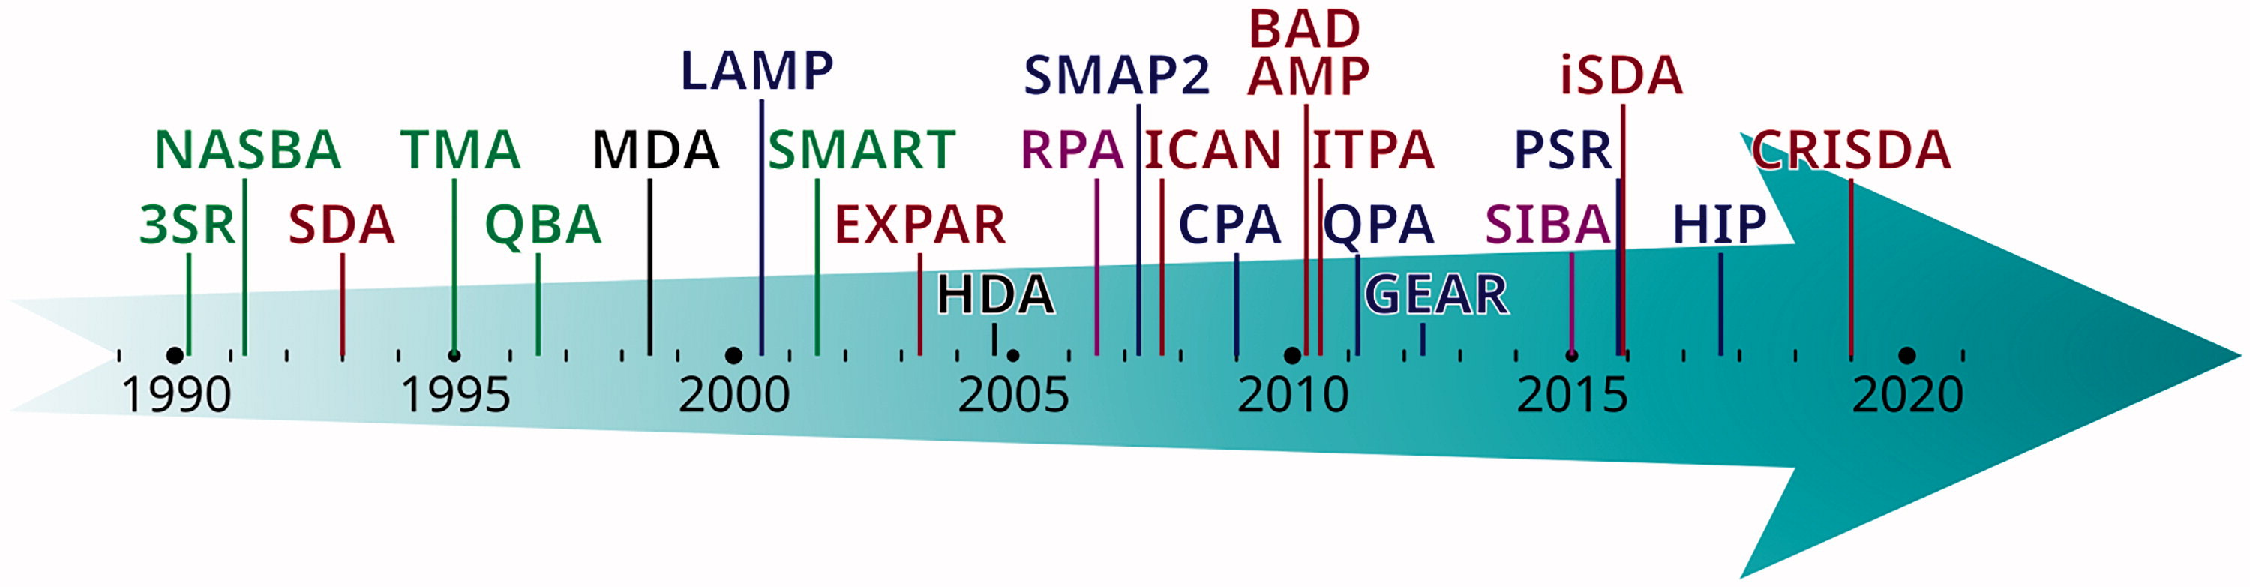
\includegraphics[width=1\textwidth]{data/iso_amp_methods.pdf}
    \caption[Timeline of isothermal nucleic acid amplification methods.]{Timeline of isothermal nucleic acid amplification methods. The colour of the amplification method indicates the underlying mechanism; promoter-based in green, nicking-based in red, refolding-based in blue, strand-invasion-based in purple and unique mechanisms in black. Image taken from Glökler et al. 2021\cite{glokler_isothermal_2021}.}
    \label{fig:iso_amp_methods}
\end{figure}

The first modern (post-PCR era) isothermal amplification method that gained attention was the self-sustained sequence replication (3SR) published in 1990 \cite{guatelli_isothermal_1990} shortly followed by the very similar nucleic acid sequence-based amplification (NASBA) in 
1991 \cite{compton_nucleic_1991} and the transcription-mediated amplification (TMA) in 1995 \cite{kacian_nucleic_1995}. They paved the way for the more than 20 isothermal amplification methods existing nowadays. The most important ones, and their working principle, are illustrated in Figure 1.2 \cite{glokler_isothermal_2021}.


%Broad explanation of isothermal amplifications
Isothermal amplifications can be categorized in numerous ways. One possibility is to separate the iNAATs that generates new strands exponentially from the ones that produce them in a linear way. Because the iNAATs that works in an exponential way are much more powerful in terms of a quick diagnosis, they dominated the diagnosis field over the linear ones.

Another way of classifying them, more useful for understanding the bigger picture of iNAATs, separates the different techniques by their underlying working principle\cite{glokler_isothermal_2021}. \linebreak

Broadly there are four different categories, illustrated in Figure 1.3:

\begin{enumerate}
   \item \emph{Promoter-based mechanisms} include target sequences for RNA polymerases in the original sequence that led to the amplification by transcription. The most well known and documented iNAAT in this category is NASBA\cite{compton_nucleic_1991}. 
   \item \emph{Nicking-based mechanisms} employs nicking enzymes to  break one of the strands to start the replication process. The resulting 3' end, left open by the enzyme, can be later used by a polymerase to start the amplification. The original method was called Strand Displacement Amplification (SDA)\cite{ness_isothermal_2003} and inspired by it, many variants have been developed.
   \linebreak
   \linebreak
   \item \emph{Refolding-based mechanisms} employs self-priming of the amplified sequences by designing the initial primers to target two different sequences in the sample, and therefore folding back generating hairpins and initiating two different amplifications. The generation of the LAMP method by the Notomi laboratory kick-started a whole plethora of similar methods in this category\cite{notomi_loop-mediated_2000}. 
   \item \emph{Strand invasion-based mechanisms} is the most novel way to perform exponential isothermal amplification. It is based on the working principle of natural recombinases, that binds to single-stranded nucleic acids, and targets double-stranded complementary sequences by a strand invasion mechanism. The most mature technology in this category is Recombinase Primed Amplification (RPA)\cite{piepenburg_dna_2006}.
\end{enumerate}

%Image that explains the different methods
\begin{figure}[b]
    \centering
    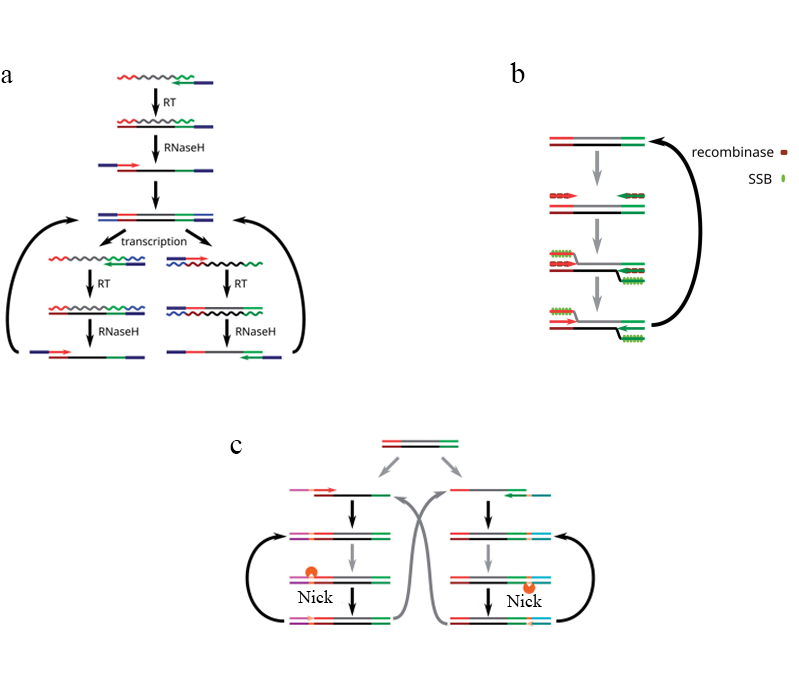
\includegraphics[width=1\textwidth]{data/iNAATs.png}
    \caption[Representation of isothermal amplification techniques]{A scheme that represents the working principles of isothermal amplification techniques based in a) promoter amplification, b) strand invasion and c) nicking enzymes. Refolding based mechanism is separated and illustrated in Figure 1.4. Image adapted from Glökler et al. 2021\cite{glokler_isothermal_2021}.}
    \label{fig:commercial iNAATs}
\end{figure}

Despite all this panorama of iNAATs developed to date, just a few of them have been significantly applied to real scenarios. In Figure 1.4 can be observed the comparison between the different tests in terms of their development state. The table A.2.1 of the appendix A gathers the main commercial kits based on iNAATs.

NASBA was one of the first techniques to not only be developed but also applied in real diagnosis scenarios. Because of its working principle, in its origins, NASBA was handy to detect viruses\cite{rutjes_real-time_2006}. A notorious recent application was its adaption to monitor the recycled water in the International Space Station\cite{bechy-loizeau_assessment_2015}. NASBA has been proven to be more sensitive and less prone to inhibitory substances than PCR\cite{rutjes_real-time_2006}, and immune to contamination by DNA, because the temperature is kept below the DNA melting point, so strand displacement does not occur\cite{simpkins_rna_2000}. Still, the high cost of the reaction (~26\$ per test\cite{oliveira_isothermal_2021}) and the need to optimize 3 different enzymes have prevented the development of commercial products based on NASBA.

\begin{figure}[b]
    \centering
    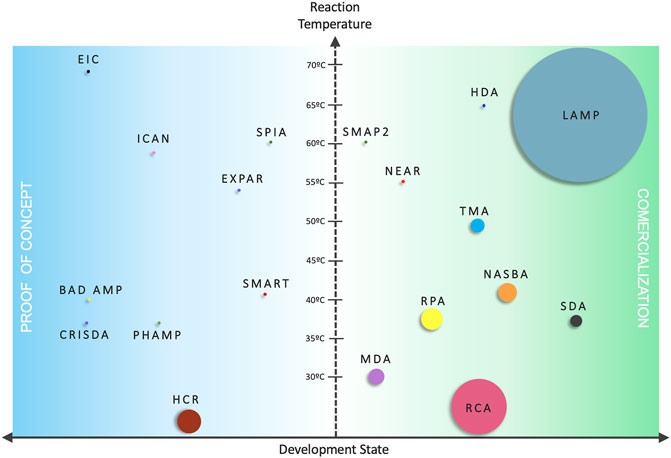
\includegraphics[width=0.85\textwidth]{figures/commercial kits.jpg}
    \caption[Comparison between iNAATs working principles and their development state.]{Comparison between iNAATs working principles and their development state. The vertical axis represents the reaction temperature and the horizontal axis how developed is the technology, from methods not developed far away from academic concepts (Blue), to already commercialized systems (Green). The size of the circles represents the number of scientific items in literature. Image obtained from Oliveira et al. 2021\cite{oliveira_isothermal_2021}.}
    \label{fig:development state}
\end{figure}

%RCA
Rolling Circle Amplification (RCA) is also one of the earlier developed iNAATs \cite{fire_rolling_1995} and even though it has some great advantages, such as the low temperature (23-60ºC) or its ability to work in complex biological matrices (allowing for molecular-level detection in living cells\cite{konry_ultrasensitive_2011}) the linear amplification profile has prevented RCA-based products to reach the diagnosis market.

%RPA
Nowadays RPA is one of the iNAATs that have more potential to win the race for the next "Gold Standard" in nucleic acid amplification \cite{oliveira_isothermal_2021}. Some of the key characteristics that justify the bloom of RPA are the low incubation temperature (37-42ºC), a PCR level sensitivity (Limit of Detection (LoD) between 10-20 copies of target DNA) and one of the fastest times-to-complete reactions (10-20 mins)\cite{kunze_-chip_2016}. Moreover, RPA assays can work with low sample volumes, seems to be robust under high concentrations of PCR inhibitors, and don't require an initial DNA denaturalization step\cite{twist_dx_recombinase_2017}\cite{kersting_rapid_2014}\cite{deng_bioanalytical_2015-1}.

These characteristics made RPA be one of the iNAATs that have the larger commercial potential. Indeed, the technology was already patented in 2005 by TwistDx (later acquired by Abbott Diagnostics). The ambit of application was originally the US and soon they expanded to the rest of the world\cite{armes_recombinase_2007}.

Apart from the patented commercialization, RPA has some limiting factors for its applicability. The fact that RPA uses a complex mix of 3 enzymes makes the system less stable and prone to lose efficiency, getting the enzymes degraded over time. Furthermore, the requirement of 3 enzymes, makes the systems complex to optimize and produce. 

Following the lessons learnt from the SARS-CoV-2 pandemic, if global needs are to be met, we cannot rely only on manufacturers primarily in high-income countries (HICs) \cite{medecins_sans_frontieres_local_2021}. 

The fact that not only one but three enzymes need to be produced, characterized and optimized, make RPA far from a short or mid-term global applicability. A simpler system, with the same potential but dependent on fewer enzymes, is required.

\section{Loop-Mediated Isothermal Amplification}

%Breve introduccion a LAMP
Loop-Mediated Isothermal Amplification (LAMP)\cite{notomi_loop-mediated_2000} is the most widely spread iNAAT, referenced in approximately 3700 scientific publications and 17 clinical trials\cite{clinicaltrialsgov_loop-mediated_2022}. Perhaps one of the most relevant acknowledgements along all the LAMP history has been its recognition by the World Health Organization to fulfil all the requirements for an \emph{ideal} diagnostics NAAT\cite{wong_loop-mediated_2018}.

%Principio de amplificación.
%Mejora con seis Primers

The working principle of LAMP can be included in the above categorization as a \emph{strand refolding mechanism} and is exemplified in Figure 1.5. LAMP relies on the strand-displacement activity of a DNA polymerase (Traditionally the Bst polymerase\cite{notomi_loop-mediated_2000}) and a special set of 4 different primers targeting 6 different regions. This is possible due to the special design of the so-called "Inner primers", composed of two sequences that align with different regions in the target strand, one in the forward sequence and the other in the reverse, and an optional separating sequence between them. Within the amplification, the inner primers re-align with their own strand, self-priming and generating a new origin of amplification. The second pair of primers, the forward and reverse outer primers, align in the external regions of the amplicon promoting the displacement of the inner primers amplified product and speeding up the reaction. 

\begin{figure}[b]
    \centering
    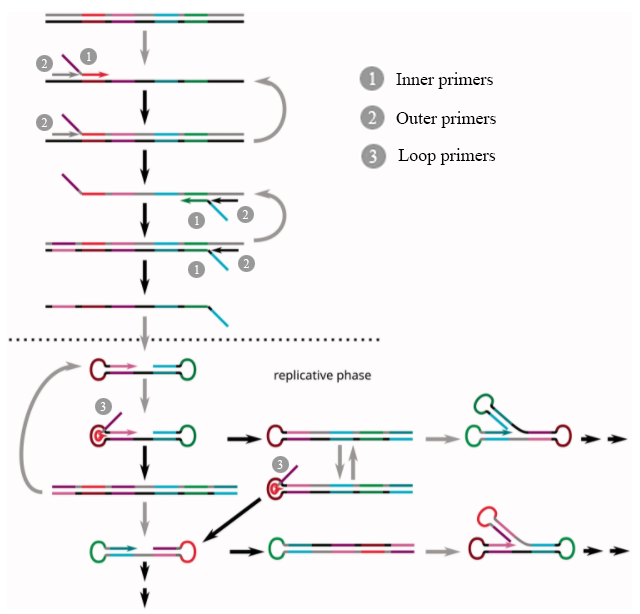
\includegraphics[width=0.8\textwidth]{figures/lamp.png}
    \caption[Explanation of the LAMP working principle.]{Explanation of the LAMP working principle. Image adapted from Glökler et al. 2021 \cite{glokler_isothermal_2021}}.
    \label{fig:LAMP}
\end{figure}

This loop-based elongation generates many different concatemeric sequences with multiple origins of amplification, that in three-dimension acquire a cauliflower shape and possess a high resistance against degradation. In a later improvement of the technique, a third pair of primers were included. These primers target the loop region generated by the Inner primers, highly accelerating the reaction\cite{nagamine_accelerated_2002}.
%Figura de como funciona y leyenda de cada primer

%Caracteristicas
This principle of work endows LAMP with the ability to detect 1 copy per microliter\cite{zhang_lamp---chip_2019}, 10 to 100 fold more sensitive than PCR, with an amplification time of less than 1h around 63-65ºC and yielding $10^9$ copies\cite{notomi_loop-mediated_2000}. Furthermore, LAMP is resistant to inhibitory substances and doesn't require, like many other iNAATs, an initial denaturation step at 95ºC\cite{enomoto_rapid_2005}\cite{kaneko_tolerance_2007}.
%Aplicación
When it comes to the applicability, the original family of LAMP patents recently expired\cite{tsugunori_notomi_hase_tetsu_process_2000}, coinciding with  the beginning of the global SARS-CoV-2 pandemic. Indeed, just within the framework of the pandemic, at least 13 diagnosis kits based in LAMP have addressed the \emph{In Vitro Diagnosys} (IVD) certification at least  in one of the main regulatory agencies in the world \cite{find_sars-cov-2_2022}, and 4 more are in development \cite{find_sars-cov-2_2022-1}. In the global infectious diseases panorama, LAMP kits have been commercialized for Tuberculosis, Malaria and Leishmania among others\cite{oliveira_isothermal_2021}. 

To summarize, there is an exponential growth of the LAMP applications and a market in expansion, partially boosted by the pandemic need for simpler and more affordable diagnosis methods. 

\section{The problem of false positives}

Even though the above-mentioned advantages, traditional LAMP face a main obstacle to being implemented; When it comes to the real application the reactions can easily come out as false positives. This problem has been partially linked with carryover contamination by the highly-stable cauliflower-shaped LAMP amplicons\cite{gao_pullulan_2019} as well as the aberrant  amplification started by secondary structures originated by the complex mix of six primers. 

Another important factor in the generation of false positives is the Bst polymerase structure. As the polymerase works at high magnesium concentrations (4-8mM) the binding between the enzyme and the substrate is allowed to be more flexible, therefore giving the Bst the ability to amplify a broader number of substrates. When it comes to the diagnosis this has pros and cons. On one hand, the Bst polymerase can amplify a broader number of nucleic acids templates (as RNA or non-standard nucleic acids) even in the presence of amplification inhibitors\cite{glokler_isothermal_2021} which allows, for example, a robust viral RNA amplification by the so-called \emph{Reverse Transcription} LAMP. On the other hand, this contributes to the so-called false positives, as the polymerase is described to not only perform non-specific amplifications but even \emph{ab initio} synthesis\cite{zyrina_ab_2014}.

Apart from the above-mentioned origins of contamination, the false positive is amplified by the traditional LAMP signal generation methods. The initially proposed method consists of the direct naked-eye observation of turbidity generation, created by the high yields of LAMP amplified DNA \cite{notomi_loop-mediated_2000}. This is not only a difficult task for the human eye, that introduce a relevant human error in the system, but also a process that will give a positive result independently of the amplified DNA sequence in the tube.

As the DNA amplification results in a PH change, PH indicators (typically phenol red) can be used to get a positive signal once the amplification is performed. This method has been used as a standard in the LAMP industry for the last years and is the one applied in the NEB WarmthStart kit\cite{new_england_biolabs_warmstart_2022}, the most spread MasterMix across laboratories. This method is not only sensible to unspecific off-target amplification but it is also described to be affected by external factors as the sample composition\cite{uribe-alvarez_low_2021}.

Intercalant dyes, commonly used in PCR-based amplification, can inhibit the amplification as they partially bind to the DNA at the incubation temperature. Even if some intercalant dyes have been described to avoid the inhibition (SYTO9/SYTO82)\cite{oscorbin_comparison_2016} the problem of unspecific signal generation is still there.

Apart from the impact in the method specificity, this unspecific amplification  further means that the above detection techniques cannot be multiplexed, eventually allowing the detection of more than one target in a single reaction. 

Other techniques have been developed based on strand displacement of a quencher bound to a probe targeting the loop region of the amplicon (DARQ\cite{tanner_simultaneous_2012} and OSD\cite{bhadra_high-surety_2020}) mimicking the working mechanism of the PCR TaqMan probes technology. The problem of these techniques is the risk of inhibiting the reaction, as the sequences used for generating the signal compete with the ones used for amplification\cite{ball_quenching_2016}.

All the above-mentioned difficulties settled the basis for the need for a specific LAMP amplification method.

\section{Quenching of Unincorporated Amplification Signal Reporters LAMP}

Quenching of Unincorporated Amplification Signal Reporters LAMP (QUASR-LAMP) is a target-specific method for generating a signal out of a LAMP amplification. QUASR-LAMP can be considered as an evolution of the above mentioned DARQ. It uses the same principle but takes advantage of quencher probes designed with lower melting temperature (Tm) that don't inhibit the reaction and keep more signal to noise ratio\cite{ball_quenching_2016}.

In Figure 1.6, the QUASR-LAMP working principle is exemplified. A fluorophore is attached to the 5' end of one of the 6 primers. A probe is designed to be complementary to the fluorescent probe with a melting temperature significantly lower than the reaction one (At least 5 ºC less)\cite{ball_quenching_2016}. In the absence of a specific amplified target, the probe keeps joined to the quencher, and the fluorescence is inhibited. When the target is amplified, its complementarity for the fluorescent probe is considerably more significant than the quenching probe, displacing their alignment and separating the quencher from the fluorophore and generating the signal. Different targets can be multiplexed with different fluorescence colours.

Combining the simplicity and affordability of the iNAATs, together with the specificity and sensitivity of PCR, QUASR-LAMP has all the characteristics required for a robust diagnose test. Alongside a proper hardware, that allows both the incubation and analysis of the reactions, the potential of QUASR-LAMP is huge and spread in fields such as infectious disease diagnosis for human health and agriculture, water purity testing and food safety analysis among others.

\begin{figure}[h]
    \centering
    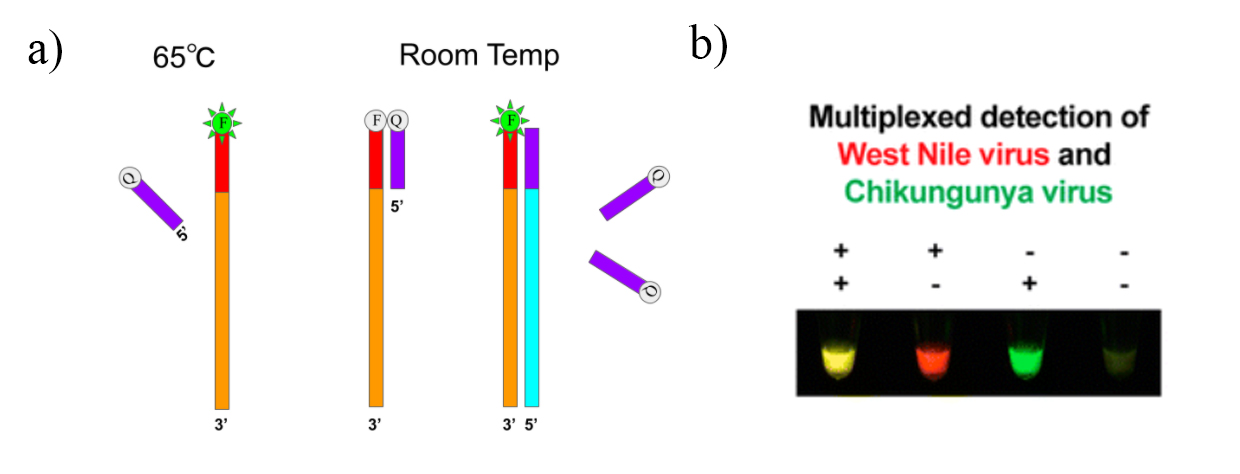
\includegraphics[width=1\textwidth]{figures/QUASR.JPG}
    \caption[Graphical summary of the QUASR-LAMP principle]{a) Graphical summary of the QUASR-LAMP principle, exemplifying the interaction between the fluorescent probes (F) the quencher (Q) and the target strand.b) Example result of a multiplexed QUASR-LAMP amplification for West Nile and Chikungunya viruses. Adapted from Ball et al. 2016\cite{ball_quenching_2016}.}
    \label{fig:QUASR}
\end{figure}

\newpage
\section{Diagnostics where are needed}
In 2019 3.2 million humans died in Low and Middle-Income Countries (LMIC) out of communicable diseases\cite{institute_for_health_metrics_and_evaluation_ihme_uniersity_of_washington_gbd_2015}, the part of the disorders that can be transmitted between individuals. This number may appear irrelevant when it is compared with the global population of 7.7 billion people\cite{worldometer_worldometer_2022} but is 7 times larger than the ones belonging to their High-Income neighbours (Figure 1.7). 

Part of this problem resides in the lack of an early diagnosis. Without them, the local healthcare regulators cannot make informed decisions based on epidemiological data. The overwhelming difference in the amount of performed diagnoses between world regions can be graphically observed in Figure 1.8 and should make us re-think how we design and deploy the current diagnosis technologies. 

Letting the price aside, an important variable contributing to this difference between regions is the massive bottleneck that the current diagnoses supply chains face to deploy the tests at LMIC. Because the production is generally centred in High-Income Countries (HICs), factors like the required cold-chain, the difficulties in the export/import custom protocols and the competition of the global market demand usually make the LMICs forgotten. In the words of the 2020 Medics Sans Frontiers access campaign \cite{medecins_sans_frontieres_local_2021}:
\\
\begin{quote}
\emph{We cannot rely only on manufacturers primarily in high-income countries (HICs) if global needs are to be met. In light of growing recognition of Low and Middle-Income Countries (LMICs) needs and accompanying efforts to increase access to diagnostics in these countries through improved local production}
\end{quote}
\vspace{20pt}

We started this project believing that QUASR-LAMP will become a game-changer in low resource diagnosis, not only because it is superior to the current gold standard in price and simplicity (with comparable robustness), but also because of the modest amount of infrastructure required, that made us glimpse its local production in the short-term.

\begin{figure}[ht]
    \centering
    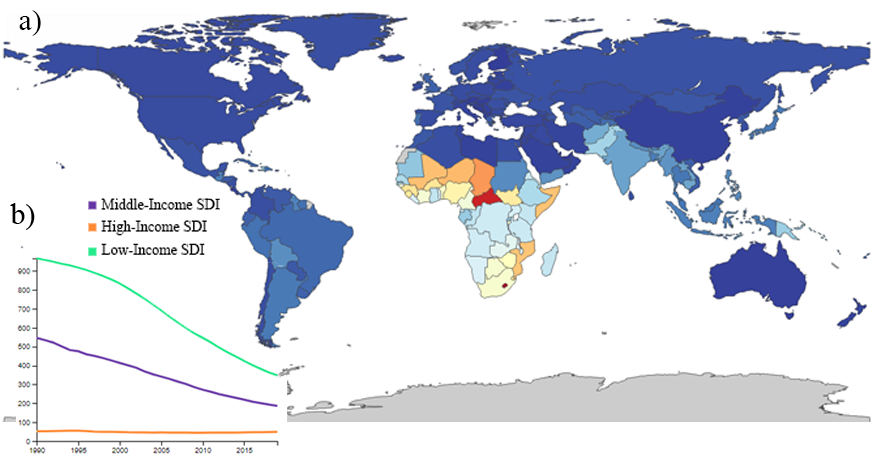
\includegraphics[width=1\textwidth]{figures/Deaths map.png}
    \caption[Summary of world rate deaths burden associated with communicable diseases.]{a) World map representing deaths rate per 100.000 population associated with communicable diseases b) Evolution of the death rate [1990 to 2020]. Adapted from GBD Compare\cite{institute_for_health_metrics_and_evaluation_ihme_uniersity_of_washington_gbd_2015}.}
    \label{fig:Deaths}
\end{figure}
\begin{figure}[b]
    \centering
    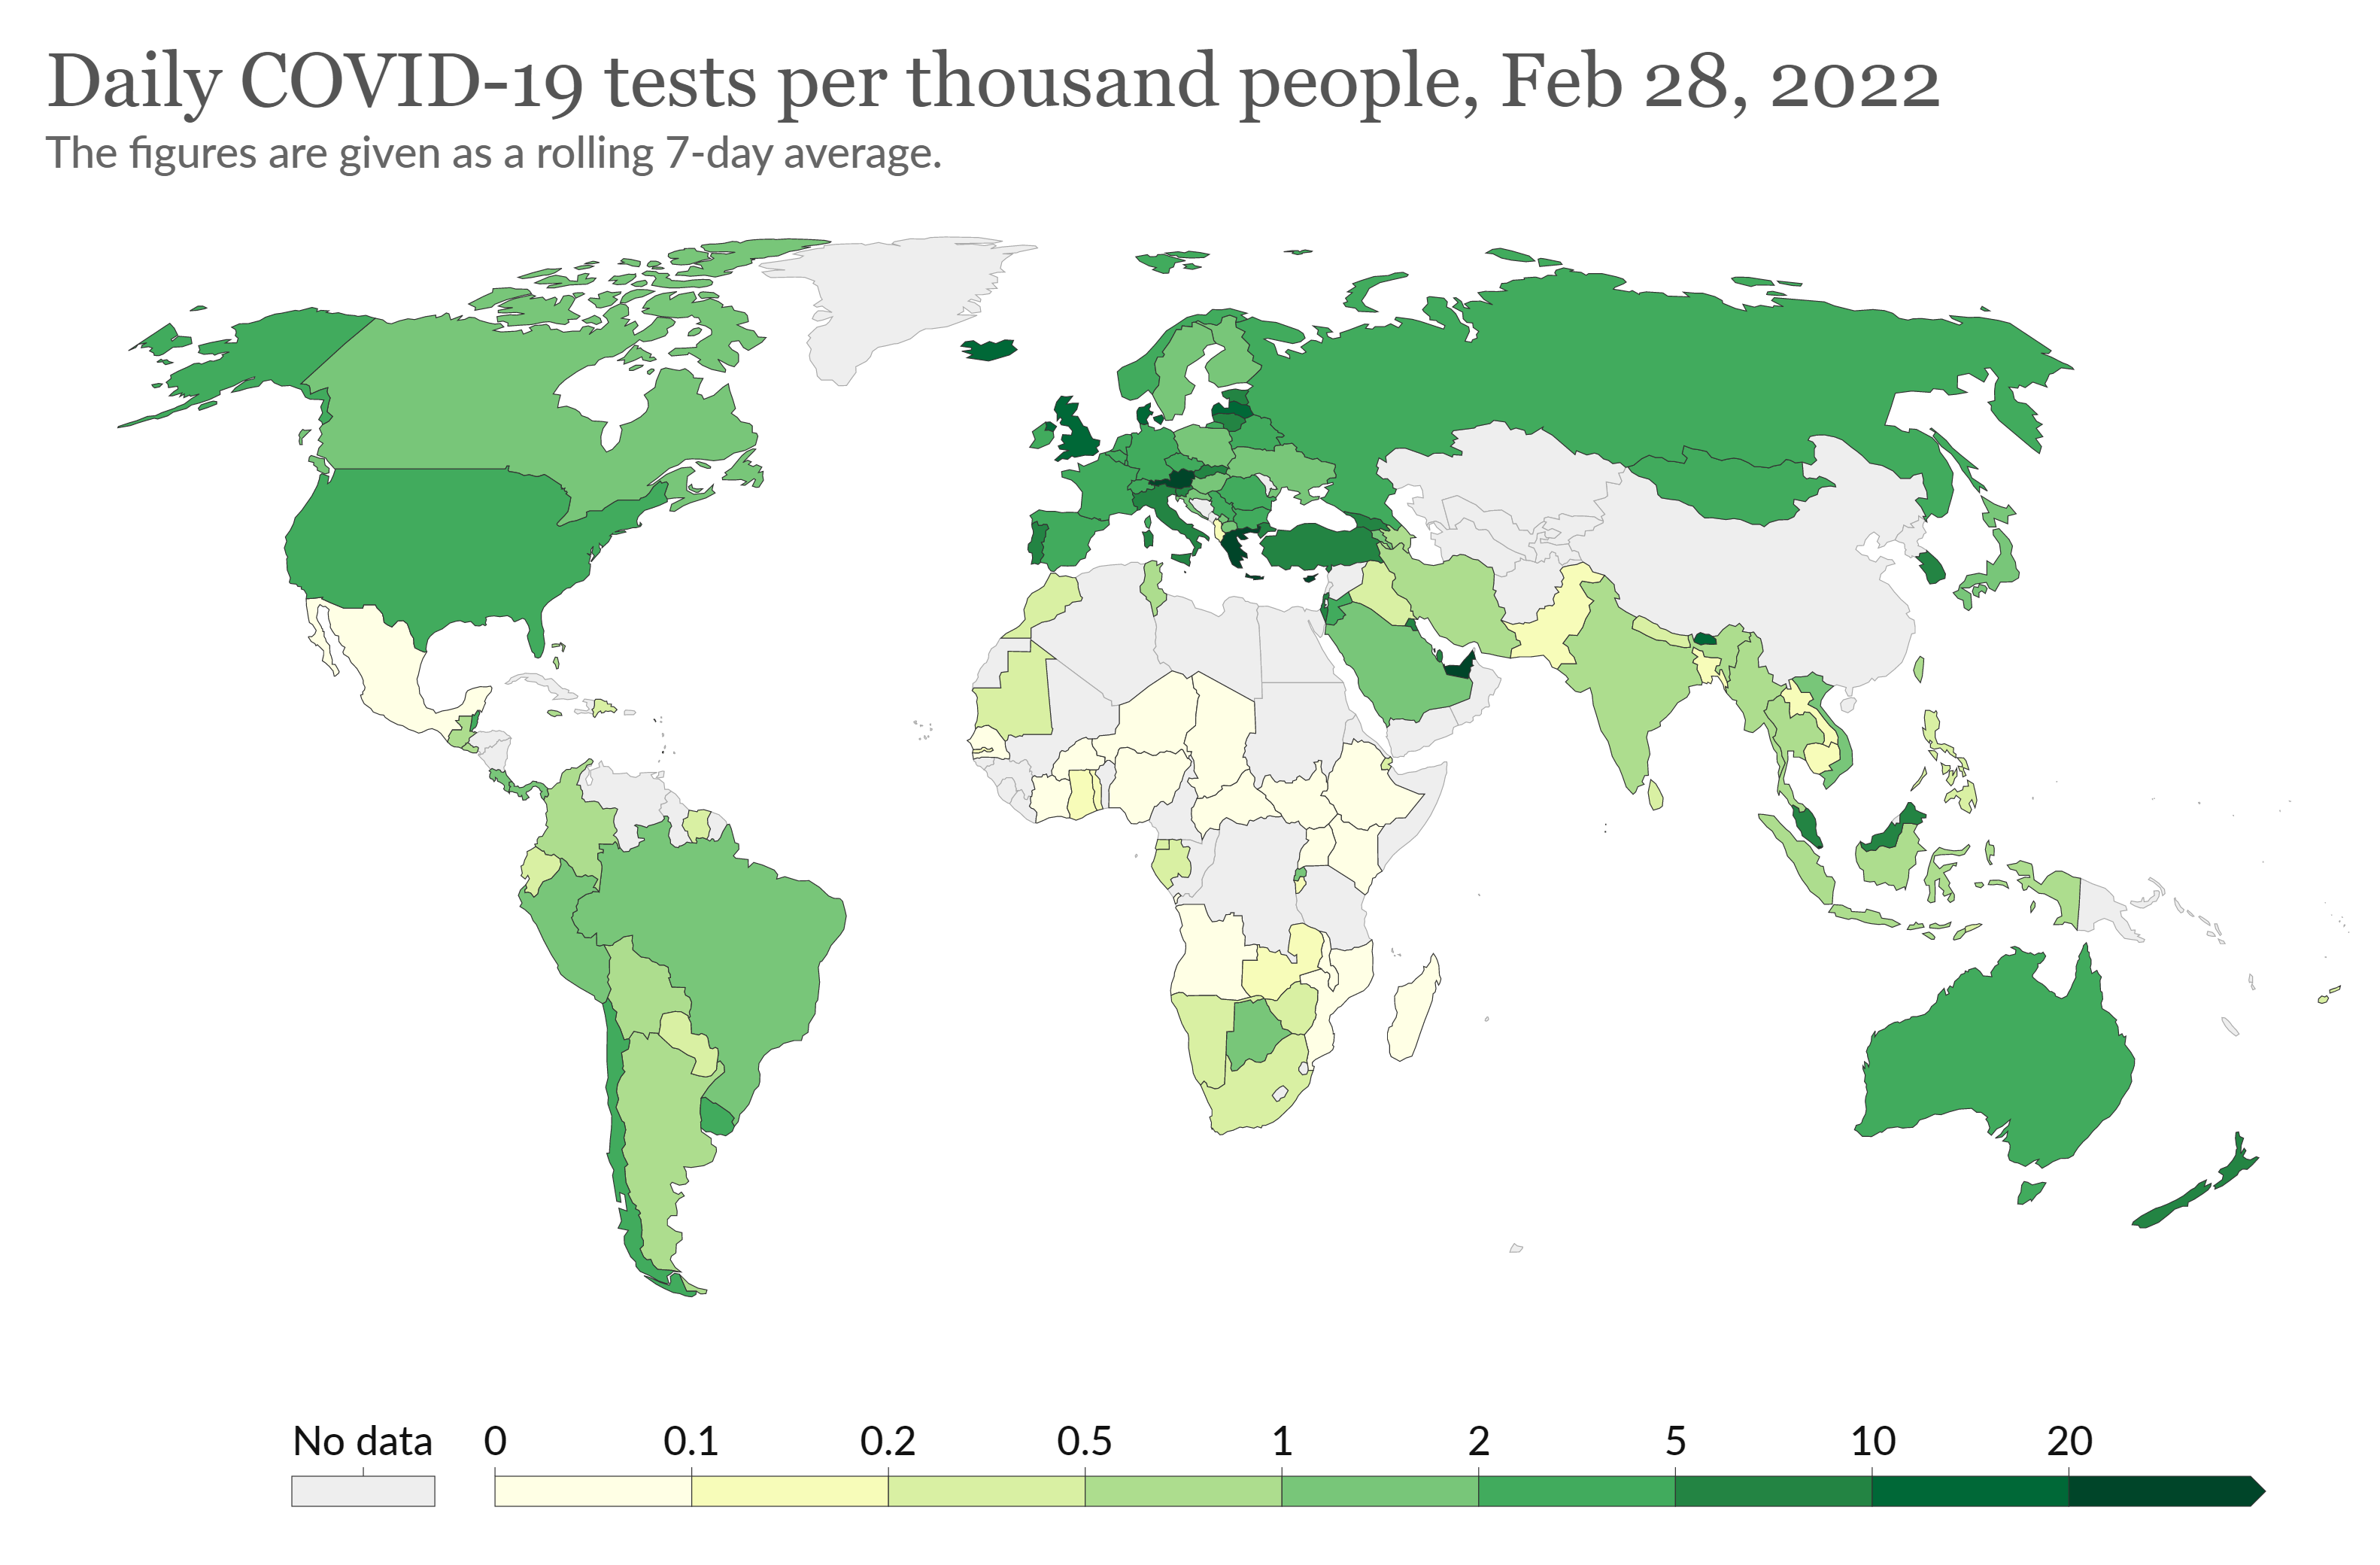
\includegraphics[width=1\textwidth]{figures/diagnosis map.png}
    \caption[World map: total tests performed relative to the size of population.] {World map: total tests performed relative to the size of population. Adapted from Our World In Data\cite{ritchie_coronavirus_2020}.}
    \label{fig:Diagnosis}
\end{figure}
\newpage
\section{Scope of the thesis}
Despite all the challenges faced during the pandemic, I always tried to overcome the problems for staying solid in the original thesis idea. The difficulties that LMICs have always faced to manufacture and deploy diagnosis tests are, since long ago, a meaningful world-challenge at a personal level. In 2019, thanks to my experience coordinating the former Madrid 2019 iGEM team\cite{igem_madrid_2019_aegis_2019}, I had the opportunity to work in Cameroon for a summer, to test our recently developed cholera sensor on the field. During this period, I had the chance to better understand the local communities, their problems and needs. It helped me to deeply interiorize the importance of constructing a world where, starting with healthcare, we all have equally satisfied our basic needs. 

During the SARS-CoV-2 pandemic, as I was not allowed to come back to Tsinghua, I reinvented my thesis plan to adapt it to the new times. I established a collaboration between Tsinghua, Cambridge and Paris universities. In the framework of this collaboration, I travelled to the Centre de Recherches Interdisciplinaires (CRI) in Paris to start using a previous technology I have worked with, QUASR-LAMP, creating a kit that would enable developing regions to perform a high throughput screening on SARS-CoV-2. The idea has always been that, once the pandemic ends, we can adapt these tools  to other communicable diseases for the long-term sake of these regions.

\vspace{12pt}
Following this vision, I defined three main goals for the present thesis:
\vspace{8pt}
\begin{enumerate}
   \item \emph{Adapt the QUASR-LAMP technology to detect the SARS-CoV-2 viral genome.}
   \item \emph{Establish an in-house production of lyophilized reactions that do not require cold chain transportation and storage. Try the system with real clinical samples on the field.}
   \item \emph{Create an affordable hardware that allows incubating and analyzing the results both qualitatively and quantitatively, keeping in mind the resource restrictions of the developing regions.}
\end{enumerate}